\documentclass[aspectratio=169]{beamer}
\usetheme[pageofpages=de,% String used between the current page and the
                         % total page count.
          alternativetitlepage=true,% Use the fancy title page.
          % titlepagelogo=trinity-stacked-full,% Logo for the first page.
          watermark=trinity-stacked,% Watermark used in every page.
          watermarkheight=50px,% Height of the watermark.
          watermarkheightmult=1,% The watermark image is 4 times bigger
                                % than watermarkheight.
          ]{Torino}

% Nouvelle is a green and red alternative to the chameleon color theme.
\setbeamercovered{invisible}
\usecolortheme{nouvelle}%
\usepackage[T1]{fontenc}
\usepackage[utf8]{inputenc}
\usepackage{graphicx}
\usepackage{tikz}
\usetikzlibrary{positioning,shapes.geometric}
\usepackage{listings}
\usepackage{xcolor}

% Configuração para JavaScript
\lstdefinelanguage{JavaScript}{
  keywords={break, case, catch, continue, debugger, default, delete, do, else, finally, for, function, if, in, instanceof, new, return, switch, this, throw, try, typeof, var, let, while, with},
  morecomment=[l]{//},
  morecomment=[s]{/*}{*/},
  morestring=[b]',
  morestring=[b]"
}

\lstset{
   language=JavaScript,
   extendedchars=true,
   basicstyle=\footnotesize\ttfamily,
   showstringspaces=false,
   showspaces=false,
   numbers=left,
   numberstyle=\footnotesize,
   numbersep=8pt,
   tabsize=2,
   breaklines=true,
   showtabs=false,
   captionpos=b
}

\usepackage{fancyvrb}

% Define um novo ambiente 'mysmallverbatim' que ajusta o tamanho da fonte para 'small'
\DefineVerbatimEnvironment%
{mysmallverbatim}{Verbatim}
{fontsize=\small}
% \usepackage[pdftex]{graphicx}  

\usepackage[portuguese]{babel}

%--------------------------------------

%Portuguese-specific commands
%--------------------------------------
\usepackage[portuguese]{babel}
%--------------------------------------

%---------------------------------------------------------------------------------
% packages
%---------------------------------------------------------------------------------
\usepackage{verbatim}
\usepackage{tikz}
\usetikzlibrary{arrows,positioning}
\usepackage{preview}
\PreviewEnvironment{tikzpicture}
\usepackage{listings}
\usepackage{amssymb}
\usepackage{xcolor, soul}

\sethlcolor{lightgray}
\newcommand{\mycode}[1]{\textcolor{red}{\hl{\texttt{#1}}}}
% \newcommand{\mycode}[1]{\textcolor{red}{\texttt{#1}}}



\author{Prof. Artur Oliveira}
\institute{Sistemas de Informação - CPAN/UFMS}

% \date{\today} % Date, can be changed to a custom date

\begin{document}

% \begin{frame}
% \titlepage
% \end{frame}


% \title{Rubro Negra}
\date{\today}
\frame{\titlepage}
% \chapter{Árvores Rubro-Negras}
\begin{frame}[fragile] 
  \frametitle{Árvore Rubro-Negra}
  \begin{theorem}
    Uma árvore rubro-negra é uma árvore binária de busca balanceada na 
    qual cada nó interno tem dois filhos. Cada nó interno tem uma cor, 
    tal que:
    
    \begin{itemize}
    \item Árvore balanceada
    \item Trata cada nó como preta ou vermelhos
    \item Cada vez que adicionamos um nó, conferimos a árvore com as regras da ARN.
    \item Dependendo da violação das regras, faremos uma inversão de cores ou rotação para corrigir os erros na árvore
    \end{itemize}
    \end{theorem}
    
    Precisamos adaptar as operações de inserção e deleção de forma que as 
    propriedades rubro negras sejam mantidas.
\end{frame}
    

%%%%%%%%%%%%
%% FRAME %%%
%%%%%%%%%%%%

\begin{frame}[fragile]{Árvore Rubro-Negra - Regras}
  \begin{theorem}
  
  \begin{itemize}
  \item[0.] Cada nó é preto ou vermelho 
  \item[1.] O nó raiz é sempre preto.
  \item[2.] Todos os nós folha (Null) são pretos.
  \item[3.] Novas inserções são sempre vermelhas.  
  \item[4.] Todos os caminhos percorridos na árvore contém o mesmo número de nós pretos (\textbf{\emph{altura-negra}}).
  \item[5.] Nenhum caminho pode ter dois nós vermelhos consecultivos. 
  \item[6.] Se um nó é vermelho, então ambos os filhos são pretos. 
  \item[7.] Os ponteiros dos nós folha (representados como quadrados pretos) continuam sendo "nulos" e não carregam nenhum valor.
  \end{itemize}
  \end{theorem}
  
\end{frame}


\begin{frame}[fragile]

    \begin{figure}[!h]
      \centering
      \caption{Típica árvore rubro-negra} 
    % \begin{preview}
    \begin{tikzpicture}[->,>=stealth',
      % level/.style={sibling distance = 8cm/#1, level distance = 1.5cm},
      level 1/.style={sibling distance=0.4\textwidth, level distance = 0.8cm},
      level 2/.style={sibling distance=0.2\textwidth, level distance = 0.8cm},
      level 3/.style={sibling distance=0.1\textwidth, level distance = 0.8cm},
      level 4/.style={sibling distance=0.05\textwidth, level distance = 0.8cm}]
    \node [bbv] (r){6}
    child {node [brv] {3}
      child {node [bbv] {1}
        child {node [nil] {}}
        child {node [nil] {}}
      }
      child {node [bbv] {5}
        child {node [nil] {}}
        child {node [nil] {}}
      }
    }
    child {node [brv] {8}
      child {node [bbv] {7}
        child {node [nil] {}}
        child {node [nil] {}}
      }
      child {node [bbv] {9}
        child {node [nil] {}}
        child {node [brv] {10}
          child {node [nil] {}}
          child {node [nil] {}}
        }
      }
    }
    ;
  \end{tikzpicture}
  \end{figure}
\end{frame}

%%%%%%%%%%%%
%% FRAME %%%
%%%%%%%%%%%%
\begin{frame}[fragile]
  \frametitle{Regras pra corrigir a árvore}

  \begin{itemize}
    \item \textbf{Tio Preto} - Rotaciona (TPR)
    \item \textbf{Tio Vermelho} - inverte cor (TVI)
  \end{itemize}

\begin{figure}
\begin{minipage}[t]{0.48\linewidth}
\centering
\caption{Resultado da TPR}
\begin{tikzpicture}[->,>=stealth',
  level 1/.style={sibling distance=6em, level distance = 3em},
  level 2/.style={sibling distance=2em, level distance = 3em},
  level 3/.style={sibling distance=1em, level distance = 3em}
]
\node [bbv] (r){c}
    child [color=black] {node [brv] {a}}
    child [color=black] {node [brv] {c}}
;
\end{tikzpicture}
\end{minipage}\hfill
\begin{minipage}[t]{0.48\linewidth}
\caption{Resultado da TVI}
  \begin{tikzpicture}[->,>=stealth',
  level 1/.style={sibling distance=6em, level distance = 3em},
  level 2/.style={sibling distance=2em, level distance = 3em},
  level 3/.style={sibling distance=1em, level distance = 3em}
]
\node [brv] (r){c}
    child [color=black] {node [bbv] {a}}
    child [color=black] {node [bbv] {c}}
;
\end{tikzpicture}
\end{minipage}
\end{figure}
\end{frame}


%%%%%%%%%%%%`'
%% FRAME %%%
%%%%%%%%%%%%

\begin{frame}[fragile]{Caso 1 - O tio de \textbf{a}, (\textbf{d}), é vermelho}
TVC - tio-vermelho-colorir 
Então como a gente faz pra corrigir a quebra de invariante (coloração rubro-negra?) 

É o que vamos ver agora!
\begin{figure}
\begin{minipage}[t]{0.48\linewidth}
\centering
\caption{Antes}
\begin{tikzpicture}[->,>=stealth',
  level 1/.style={sibling distance=6em, level distance = 3em},
  level 2/.style={sibling distance=2em, level distance = 3em},
  level 3/.style={sibling distance=1em, level distance = 3em}
]
\node [bbv] (r){c}
child [color=black] { node [brv] {b}
        child [color=black] {node [bwv] {z}}
        child [color=black] { node [brv] {a}
          child [color=black] {node [bwv] {x}}
          child [color=black] {node [bwv] {y}}
        }
      }
child [color=black] { node [brv] {d}
        child [color=black] {node [bwv] {p}}
        child [color=black] {node [bwv] {q}}
};
\end{tikzpicture}
\end{minipage}\hfill
\begin{minipage}[t]{0.48\linewidth}
\caption{Depois}
  \begin{tikzpicture}[->,>=stealth',
  level 1/.style={sibling distance=6em, level distance = 3em},
  level 2/.style={sibling distance=2em, level distance = 3em},
  level 3/.style={sibling distance=1em, level distance = 3em}
]
\node [brv] (r){c}
child [color=black] { node [bbv] {b}
        child [color=black] {node [bwv] {z}}
        child [color=black] { node [brv] {a}
          child [color=black] {node [bwv] {x}}
          child [color=black] {node [bwv] {y}}
        }
      }
child [color=black] { node [bbv] {d}
        child [color=black] {node [bwv] {p}}
        child [color=black] {node [bwv] {q}}
};
\end{tikzpicture}
\end{minipage}
\end{figure}
\end{frame}

%%%%%%%%%%%%
%% FRAME %%%
%%%%%%%%%%%%

\begin{frame}[fragile]{Caso 2 - O tio de \textbf{a}, (\textbf{d}), é preto e \textbf{a} é filho direito}
TPR - tio-preto-rotaciona
% \pagebreak
\begin{itemize}
  \item Rotação à esquerda do pai de \textbf{a}, (\textbf{b}), ao redor de \textbf{a}
  \item Continua para o \textbf{Caso 3}
\end{itemize}

\begin{columns}[T] % align columns
  \begin{column}{.48\textwidth}
  \rule{\linewidth}{4pt}
  \begin{figure}[!h]
  \caption{Antes}
\begin{tikzpicture}[->,>=stealth',
  % level/.style={sibling distance = 20em, level distance = 3em},
  level 1/.style={sibling distance=6em, level distance = 3em},
  level 2/.style={sibling distance=3em, level distance = 3em},
  level 3/.style={sibling distance=2em, level distance = 3em}
]
\node [bbv] (r){c}
child [color=black] { node [brv] {b}
        child [color=black] {node [bwv] {x}}
        child [color=black] { node [brv] {a}
          child [color=black] {node [bwv] {y}}
          child [color=black] {node [bwv] {z}}
        }
      }
child [color=black] { node [bwv] {w}};
\end{tikzpicture}
\end{figure}
   
\end{column}%
\hfill%
\begin{column}{.48\textwidth}
\rule{\linewidth}{4pt}
      
    
\begin{figure}[!h]
  \centering
  % \centering
  \caption{Depois}
\begin{tikzpicture}[->,>=stealth',
   % level/.style={sibling distance = 20em, level distance = 3em},
   level 1/.style={sibling distance=6em, level distance = 3em},
  level 2/.style={sibling distance=3em, level distance = 3em},
  level 3/.style={sibling distance=2em, level distance = 3em},
  ] 
\node [bbv] (r){c}
child [color=black] { node [brv] {a}
    child [color=black] { node [brv] {b}
      child [color=black] {node [bwv] {x}}
      child [color=black] {node [bwv] {y}}
    }
    child [color=black] {node [bwv] {z}}
}
child [color=black] { node [bwv] {w}};
\end{tikzpicture}
\end{figure}
\end{column}%
\end{columns}
\end{frame}


%%%%%%%%%%%%
%% FRAME %%%
%%%%%%%%%%%%

\begin{frame}[fragile]{Caso 3 - O tio de \textbf{a}, (\textbf{d}), é preto e \textbf{a} é filho esquerdo }

\begin{itemize}
  \item Rotação à direita de \textbf{c}, ao redor de \textbf{b}
  \item Troque as cores entre o pai de \textbf{b}, (\textbf{a}) e seu novo irmão (\textbf{c}).
\end{itemize}
  

\begin{columns}[T] % align columns
  \begin{column}{.31\textwidth}
  \rule{\linewidth}{4pt}
  \begin{figure}[!h]
  \caption{Antes}
\begin{tikzpicture}[->,>=stealth',
  % level/.style={sibling distance = 20em, level distance = 3em},
  level 1/.style={sibling distance=6em, level distance = 3em},
  level 2/.style={sibling distance=3em, level distance = 3em},
  level 3/.style={sibling distance=2em, level distance = 3em}
]
\node [bbv] (r){c}
child [color=black] { node [brv] {a}
    child [color=black] { node [brv] {b}
      child [color=black] {node [bwv] {x}}
      child [color=black] {node [bwv] {y}}
    }
    child [color=black] {node [bwv] {z}}
}
child [color=black] { node [bwv] {w}};
\end{tikzpicture}
\end{figure}
   
\end{column}%
\hfill%
\begin{column}{.31\textwidth}
\rule{\linewidth}{4pt}
      
    
\begin{figure}[!h]
  \centering
  % \centering
  \caption{Durante}
\begin{tikzpicture}[->,>=stealth',
   % level/.style={sibling distance = 20em, level distance = 3em},
   level 1/.style={sibling distance=6em, level distance = 3em},
  level 2/.style={sibling distance=3em, level distance = 3em},
  level 3/.style={sibling distance=3em, level distance = 3em},
  ] 
  \node [brv] (r){a}
  child [color=black] { node [brv] {b}
    child [color=black] {node [bwv] {x}}
    child [color=black] {node [bwv] {y}}
  }
  child [color=black] { node [bbv] {c}
    child [color=black] {node [bwv] {z}}
    child [color=black] {node [bwv] {w}}
  };
\end{tikzpicture}
\end{figure}
\end{column}%
%
\hfill%
\begin{column}{.31\textwidth}
\rule{\linewidth}{4pt}
      
    
\begin{figure}[!h]
  \centering
  % \centering
  \caption{Depois}
  \begin{tikzpicture}[->,>=stealth',
    % level/.style={sibling distance = 20em, level distance = 3em},
    level 1/.style={sibling distance=6em, level distance = 3em},
   level 2/.style={sibling distance=3em, level distance = 3em},
   level 3/.style={sibling distance=3em, level distance = 3em},
   ] 
   \node [bbv] (r){a}
   child [color=black] { node [brv] {b}
     child [color=black] {node [bwv] {x}}
     child [color=black] {node [bwv] {y}}
   }
   child [color=black] { node [brv] {c}
     child [color=black] {node [bwv] {z}}
     child [color=black] {node [bwv] {w}}
   };
 \end{tikzpicture}

\end{figure}
\end{column}%
\end{columns}
\end{frame}
  
% \title{Estruturas de Dados: Apresentação da Disciplina}
\date{\today}
\frame{\titlepage}

\begin{frame}
  \frametitle{Ementa da Disciplina}
  Descrição do conteúdo a ser abordado na disciplina. Este conteúdo é importado automaticamente do Plano Pedagógico do Curso (PPC) vigente. Os tópicos principais incluem:
  \begin{itemize}
    \item Tabelas de Dispersão
    \item Árvores Binárias de Busca
    \item Árvores Balanceadas
    \item Busca Digital
    \item Processamento de Cadeias: Busca de Padrão e Compactação de Dados
  \end{itemize}
  Esta ementa é projetada para fornecer uma compreensão fundamental das estruturas de dados essenciais para a computação, com um foco especial em suas aplicações práticas e teóricas.
\end{frame}

\begin{frame}
  \frametitle{Objetivos Gerais}
  A disciplina visa:
  \begin{itemize}
    \item Compreender os fundamentos e a importância das estruturas de dados, enfatizando sua relevância para a eficiência dos algoritmos e o impacto no desempenho de software.
    \item Desenvolver habilidades de análise de complexidade, capacitando os alunos a analisar a complexidade de tempo e espaço de algoritmos associados a diferentes estruturas de dados.
  \end{itemize}
\end{frame}


\begin{frame}
  \frametitle{Objetivos Específicos - Tabelas de Dispersão}
  Os alunos deverão:
  \begin{itemize}
    \item Compreender o conceito, uso e implementação de tabelas de dispersão.
    \item Analisar e aplicar técnicas de tratamento de colisões.
  \end{itemize}
\end{frame}


\begin{frame}
  \frametitle{Objetivos Específicos - Árvores Binárias de Busca}
  Os alunos deverão:
  \begin{itemize}
    \item Entender a estrutura, propriedades e operações de árvores binárias de busca.
    \item Implementar inserção, busca, remoção e percurso em árvores binárias de busca.
  \end{itemize}
\end{frame}
\begin{frame}
  \frametitle{Objetivos Específicos - Árvores Balanceadas}
  Os alunos deverão:
  \begin{itemize}
    \item Aprender sobre árvores AVL e Red-Black, suas propriedades e operações.
    \item Desenvolver habilidades para implementar e manter árvores balanceadas.
  \end{itemize}
\end{frame}

\begin{frame}
  \frametitle{Objetivos Específicos - Busca Digital}
  Os alunos deverão:
  \begin{itemize}
    \item Entender o princípio da busca digital e sua aplicação em estruturas como Tries.
    \item Implementar árvores de busca digital para otimizar a busca por cadeias de caracteres.
  \end{itemize}
\end{frame}

\begin{frame}
  \frametitle{Objetivos Específicos - Processamento de Cadeias}
  Os alunos deverão:
  \begin{itemize}
    \item Compreender e aplicar algoritmos para busca de padrão em textos.
    \item Estudar e implementar técnicas de compactação de dados.
  \end{itemize}
\end{frame}

\begin{frame}
  \frametitle{Semana 1: Introdução (04/03 - 10/03)}
  \textbf{Objetivos:} Apresentar o curso, objetivos, metodologia e avaliação. Introdução aos conceitos básicos de estruturas de dados.
  
  \textbf{Leitura Recomendada:} Capítulos introdutórios dos livros de Cormen e Ascencio.
\end{frame}

\begin{frame}
  \frametitle{Semana 2: Tabelas de Dispersão (11/03 - 17/03)}
  \textbf{Tópicos:} Conceitos básicos, funções hash, tratamento de colisões.
  
  \textbf{Prática:} Exercícios de implementação de funções hash simples.
\end{frame}

\begin{frame}
  \frametitle{Semana 3: Listas, Filas, Pilhas (18/03 - 24/03)}
  \textbf{Tópicos:} Estrutura de uma lista, e os métodos de busca, inserção e remoção.
  
  \textbf{Prática:} Implementação de listas, filas e pilhas, e reuso de funções.
\end{frame}

\begin{frame}
  \frametitle{Semana 4: Árvores Binárias de Busca - Parte 1 (25/03 - 31/03)}
  \textbf{Tópicos:} Conceitos, inserção, busca e percurso.
  
  \textbf{Prática:} Implementação de árvores binárias de busca.
\end{frame}

\begin{frame}
  \frametitle{Semana 5: Árvores Binárias de Busca - Parte 2 (01/04 - 07/04)}
  \textbf{Tópicos:} Remoção, propriedades e aplicações práticas.
  
  \textbf{Prática:} Exercícios de complexidade e otimização.
\end{frame}

\begin{frame}
  \frametitle{Semana 6: Árvores Balanceadas - AVL (08/04 - 14/04)}
  \textbf{Tópicos:} Introdução, rotações, inserção e remoção.
  
  \textbf{Prática:} Implementação de árvores AVL.
\end{frame}

\begin{frame}
  \frametitle{Semana 7: Árvores Balanceadas - Red-Black (15/04 - 21/04)}
  \textbf{Tópicos:} Conceitos, propriedades, operações.
  
  \textbf{Prática:} Implementação de árvores Red-Black.
\end{frame}

\begin{frame}
  \frametitle{Semana 8: Busca Digital (22/04 - 28/04)}
  \textbf{Tópicos:} Trie, operações básicas, aplicabilidade.
  
  \textbf{Prática:} Implementação de Tries para busca de padrões.
\end{frame}

\begin{frame}
  \frametitle{Semana 9: Revisão e Avaliação Intermediária (29/04 - 05/05)}
  \textbf{Atividades:} Primeira prova teórica/prática.
\end{frame}

\begin{frame}
  \frametitle{Semana 10: Processamento de Cadeias - Busca de Padrão (06/05 - 12/05)}
  \textbf{Tópicos:} Algoritmos de busca de padrões, KMP, Boyer-Moore.
  
  \textbf{Prática:} Implementação e análise de algoritmos de busca.
\end{frame}

\begin{frame}
  \frametitle{Semana 11: Processamento de Cadeias - Compactação de Dados (13/05 - 19/05)}
  \textbf{Tópicos:} Técnicas de compactação, Huffman, LZW.
  
  \textbf{Prática:} Implementação de algoritmos de compactação.
\end{frame}

\begin{frame}
  \frametitle{Semana 12-13: Projetos Práticos (20/05 - 02/06)}
  \textbf{Atividades:} Desenvolvimento de projetos práticos em pequenos grupos, aplicando as estruturas de dados estudadas.
\end{frame}

\begin{frame}
  \frametitle{Semana 14: Aplicações Avançadas e Estudo de Caso (03/06 - 09/06)}
  \textbf{Tópicos:} Discussão de estudos de caso, uso de estruturas de dados em sistemas reais.
\end{frame}

\begin{frame}
  \frametitle{Semana 15: Revisão Geral (10/06 - 16/06)}
  \textbf{Atividades:} Revisão de todos os tópicos, sessões de dúvidas.
\end{frame}

\begin{frame}
  \frametitle{Semana 16-17: Apresentação dos Projetos Práticos (17/06 - 30/06)}
  \textbf{Atividades:} Apresentação e avaliação dos projetos práticos. Feedback individual e em grupo.
\end{frame}

\begin{frame}
  \frametitle{Semana 18: Avaliação Final e Encerramento (01/07 - 05/07)}
  \textbf{Atividades:} Avaliação final teórica. Encerramento do curso, feedback e discussão sobre aprendizados.
\end{frame}
\begin{frame}
  \frametitle{Metodologia da Disciplina}
  A disciplina será conduzida através de:
  \begin{itemize}
    \item Aulas Expositivas: Utilização do quadro e giz, e projetor para explicar conceitos, desenhar estruturas e demonstrar algoritmos.
    \item Práticas de Programação: Exercícios em sala de aula e laboratório de computação para aplicação prática dos conceitos.
  \end{itemize}
\end{frame}
\begin{frame}
  \frametitle{Estudo de Casos e Projetos Práticos}
  A disciplina incluirá:
  \begin{itemize}
    \item Análise de Casos Reais: Discussão sobre a aplicação de estruturas de dados em problemas reais.
    \item Desenvolvimento de Projetos: Trabalho em projetos práticos em grupos para solucionar desafios complexos.
  \end{itemize}
\end{frame}
\begin{frame}
  \frametitle{Avaliação e Feedback}
  Para promover o aprendizado efetivo, será aplicado:
  \begin{itemize}
    \item Avaliações Contínuas: Quizzes, exercícios de programação e participação.
    \item Feedback Construtivo: Orientações individuais e em grupo sobre as atividades.
  \end{itemize}
\end{frame}
\begin{frame}
  \frametitle{Recursos Complementares}
  Para aprofundamento do conhecimento:
  \begin{itemize}
    \item Materiais Online e Leituras Adicionais: Artigos, tutoriais, fóruns, além das leituras dos livros-texto.
  \end{itemize}
\end{frame}
\begin{frame}
  \frametitle{Bibliografia Básica}
  Livros essenciais para o estudo da disciplina:
  \begin{itemize}
    \item ASCENCIO, Ana Fernanda Gomes. \emph{Estruturas de dados: algoritmos, análise da complexidade e implementações em Java e C/C++}. São Paulo, SP: Pearson, 2010-2012. ISBN 978-85-7605-881-6.
    \item CORMEN, Thomas H. \emph{Algoritmos: teoria e prática}. Rio de Janeiro, RJ: Elsevier, 2012. ISBN 978-85-352-3699-6.
    \item EDMONDS, J. \emph{How to Think About Algorithms}. 1.ed. Cambridge: Cambridge University Press, 2008. ISBN: 978-0521614108.
  \end{itemize}
\end{frame}
\begin{frame}
  \frametitle{Bibliografia Complementar}
  Leituras adicionais para aprofundamento:
  \begin{itemize}
    \item DEITEL, Harvey M.; DEITEL, P. J. \emph{C++: como programar}. 5. ed. Porto Alegre, RS: Bookman, 2006. ISBN 85-7307-740-9.
    \item GUSFIELD, D. \emph{Algorithms on strings trees and sequences}. Cambridge: Cambridge University Press, 1997. ASIN: B009NG2XWA.
    \item KLEINBERG, Jon; TARDOS, Éva. \emph{Algorithm design}. Boston, MA: Pearson, c2014. ISBN 0321295358.
  \end{itemize}
\end{frame}

% \title{Introdução às Tabelas de Dispersão}
\date{\today}
\frame{\titlepage}

% Slide 1: Introdução às Tabelas de Dispersão
% Slide de Introdução às Tabelas de Dispersão
% Definição e Propósito: A definição e o propósito estão bem explicados. Considerar adicionar um exemplo simples de aplicação para ilustrar melhor a utilidade das tabelas de dispersão.
% Importância: O texto está claro, mas poderia ser enriquecido com exemplos específicos de como as tabelas de dispersão contribuem para o desempenho de sistemas em cenários reais.
\begin{frame}[fragile]
  \frametitle{Introdução às Tabelas de Dispersão}
  \begin{itemize}
    \item Definição e propósito das tabelas de dispersão:
      \begin{itemize}
        \item \textbf{Definição:} As tabelas de dispersão são estruturas de dados que mapeiam chaves para valores, permitindo uma recuperação eficiente dos valores associados às chaves.
        \item \textbf{Propósito:} Elas são amplamente utilizadas em diversos campos da ciência da computação e da engenharia de software devido à sua capacidade de armazenar e recuperar dados de forma rápida e eficiente.
      \end{itemize}
  \end{itemize}
\end{frame}

\begin{frame}[fragile]
  \frametitle{Introdução às Tabelas de Dispersão}
  \begin{itemize}
    
    \item Importância no armazenamento e recuperação eficiente de dados:
      \begin{itemize}
        \item Em muitas aplicações, especialmente aquelas que envolvem grandes volumes de dados, como bancos de dados, sistemas de cache e dicionários, as tabelas de dispersão são essenciais para garantir um acesso rápido e eficiente aos dados.
        \item Elas são usadas para resolver problemas como pesquisa, indexação e associação de chaves a valores, proporcionando uma maneira eficiente de armazenar e recuperar informações.
      \end{itemize}
  \end{itemize}
\end{frame}

% Slide 2: Como Funcionam as Tabelas de Dispersão
% Slide de Como Funcionam as Tabelas de Dispersão
% Processo de Mapeamento: Considerar a inclusão de um diagrama para ilustrar o processo de conversão de chaves em índices de tabela.
% Funções Hash: O texto está claro, mas adicionar um exemplo concreto de uma função hash pode ajudar a ilustrar o conceito.
\begin{frame}[fragile]
  \frametitle{Como Funcionam as Tabelas de Dispersão}
  \begin{itemize}
    \item \textbf{Processo de mapeamento de chaves para índices de tabela:}
      \begin{itemize}
        \item Utilizam funções hash para converter chaves em índices de tabela, onde os valores associados são armazenados.
        \item O objetivo é distribuir as chaves uniformemente pela tabela, minimizando colisões e facilitando uma recuperação eficiente.
        \item \textbf{Diagrama:} [Incluir um diagrama aqui que ilustre uma chave sendo convertida em um índice de tabela através de uma função hash, destacando a distribuição uniforme das chaves.]
      \end{itemize}
    
  \end{itemize}
\end{frame}
\begin{frame}[fragile]
  \frametitle{Como Funcionam as Tabelas de Dispersão}
  \begin{figure}
    \centering
    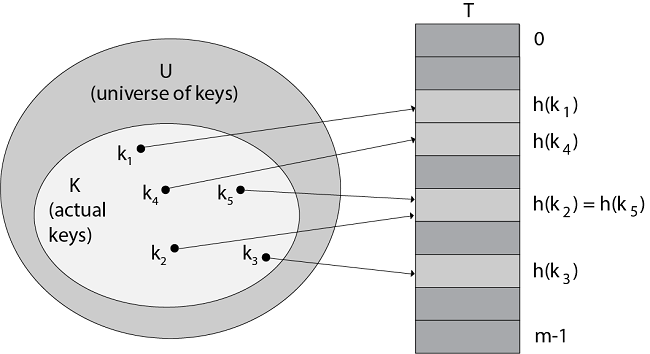
\includegraphics[width=0.8\textwidth]{aulas/aula2-hash-fig1.png}
    \caption{Caption of the Image}
  \end{figure}
\end{frame}
\begin{frame}[fragile]
  \frametitle{Como Funcionam as Tabelas de Dispersão}
  \begin{itemize}
    \item \textbf{Uso de funções hash para conversão de chaves:}
      \begin{itemize}
        \item Essenciais para a eficiência das tabelas de dispersão, as funções hash transformam chaves em índices de tabela de maneira rápida.
        \item Distribuem as chaves uniformemente, evitando colisões excessivas e otimizando o desempenho.
        \item \textbf{Exemplo Concreto:} Suponha uma função hash simples onde a chave é um número inteiro e o tamanho da tabela é 10. A função hash pode ser \(hash(k) = k \mod 10\), onde \(k\) é a chave. Se \(k = 23\), então \(hash(23) = 3\), indicando que o valor associado à chave 23 será armazenado no índice 3 da tabela.
      \end{itemize}
  \end{itemize}
\end{frame}


% Slide 3: Funções Hash
% Slide de Funções Hash
% Definição e Propriedades: A explicação está adequada. Seria útil incluir exemplos visuais para demonstrar a uniformidade e a eficiência.
% Exemplos de Funções Hash: Está bom, mas considerar adicionar exemplos de código ou pseudocódigo para as funções de hash mencionadas.
\begin{frame}[fragile]
  \frametitle{Definição e Propriedades das Funções Hash}
  \begin{itemize}
    \item \textbf{Definição:} 
      \begin{itemize}
        \item Uma função hash converte dados de tamanho variável em valores de 
        tamanho fixo, ideal para índices de tabela.
      \end{itemize}
    \item \textbf{Propriedades desejáveis:}
      \begin{itemize}
        \item \textbf{Uniformidade:} Distribui chaves de forma uniforme, 
        evitando sobrecarga em partes específicas da tabela.
        \item \textbf{Eficiência:} Rápida no cálculo, garantindo acesso ágil 
        aos dados.
        \item \textbf{Baixa probabilidade de colisão:} Minimiza casos onde 
        chaves distintas resultam no mesmo índice.
      \end{itemize}
    \item \textbf{Visualização:} Incluir um gráfico demonstrando a distribuição 
    uniforme das chaves pela tabela pode ajudar a ilustrar a uniformidade. 
    (Considerar adicionar um gráfico ou diagrama que ilustre esta propriedade.)
  \end{itemize}
\end{frame}

\begin{frame}[fragile]
  \frametitle{Exemplos de Funções Hash com Pseudocódigo}
  \begin{itemize}
    \item \textbf{Exemplos de funções hash simples com pseudocódigo:}
      \begin{itemize}
        \item \textbf{Função de Módulo:}
        \begin{mysmallverbatim}
            funcao_hash_modulo(chave, tamanho_da_tabela):
              return chave % tamanho_da_tabela
        \end{mysmallverbatim}
        \item \textbf{Função de Multiplicação:}
          \begin{mysmallverbatim}
            funcao_hash_multiplicacao(chave, tamanho_da_tabela):
              A = 0.6180339887 # constante (número de ouro - 1)
              return floor(tamanho_da_tabela * (chave * A \% 1))
          \end{mysmallverbatim}
      \end{itemize}
    \item Estes pseudocódigos ilustram métodos comuns para transformar chaves 
    em índices de tabela. A função de módulo é simples e direta, enquanto a 
    função de multiplicação utiliza uma constante para ajudar a distribuir as 
    chaves de maneira mais uniforme.
  \end{itemize}
\end{frame}




% Slide 4: Prática - Implementando Funções Hash Simples

\begin{frame}[fragile]
  \frametitle{Prática - Implementando Funções Hash Simples}
  \begin{mysmallverbatim}
    // Exemplo de função hash simples em pseudocódigo
    funcao hash(chave):
      return chave % tamanho_da_tabela
  \end{mysmallverbatim}
  \begin{itemize}
    \item A implementação acima mostra uma função hash simples que calcula o resto da divisão da chave pelo tamanho da tabela.
    \item Esta é uma abordagem comum para implementação de funções hash simples, onde a chave é mapeada diretamente para um índice na tabela.
    \item No entanto, é importante considerar que essa função pode resultar em colisões se as chaves não estiverem uniformemente distribuídas.
    \item Para testar a função hash, é recomendável utilizar uma variedade de chaves e verificar se os índices resultantes estão distribuídos de forma uniforme pela tabela.
    \item Também é importante considerar o desempenho da função hash em diferentes cenários e o impacto das colisões no desempenho geral da tabela de dispersão.
  \end{itemize}
\end{frame}


% Aula 2: Tratamento de Colisões
% Slide 1: Introdução ao Tratamento de Colisões

\begin{frame}[fragile]
  \frametitle{Introdução ao Tratamento de Colisões}
  O que são colisões e por que ocorrem?
      \begin{itemize}
        \item Colisões ocorrem quando duas ou mais chaves diferentes são mapeadas para o mesmo índice na tabela de dispersão.
        \item Elas são inevitáveis em tabelas de dispersão de tamanho fixo, especialmente quando o espaço de chaves é maior do que o número de índices na tabela.
        \item As colisões podem ocorrer devido à natureza das funções hash ou à distribuição desigual das chaves.
      \end{itemize}
\end{frame}

\begin{frame}[fragile]
  \frametitle{Introdução ao Tratamento de Colisões}
  Impacto das colisões no desempenho das tabelas de dispersão:
      \begin{itemize}
        \item Colisões podem causar uma redução significativa no desempenho das tabelas de dispersão, pois aumentam o tempo de busca e inserção de elementos.
        \item Se não forem tratadas adequadamente, as colisões podem levar a uma degradação do desempenho e a uma distribuição desigual dos elementos na tabela.
        \item Portanto, é importante implementar métodos eficazes de tratamento de colisões para garantir um desempenho ótimo das tabelas de dispersão.
      \end{itemize}
\end{frame}


\begin{frame}[fragile]
  \frametitle{Tratamento de Colisões}
  \begin{figure}
    \centering
    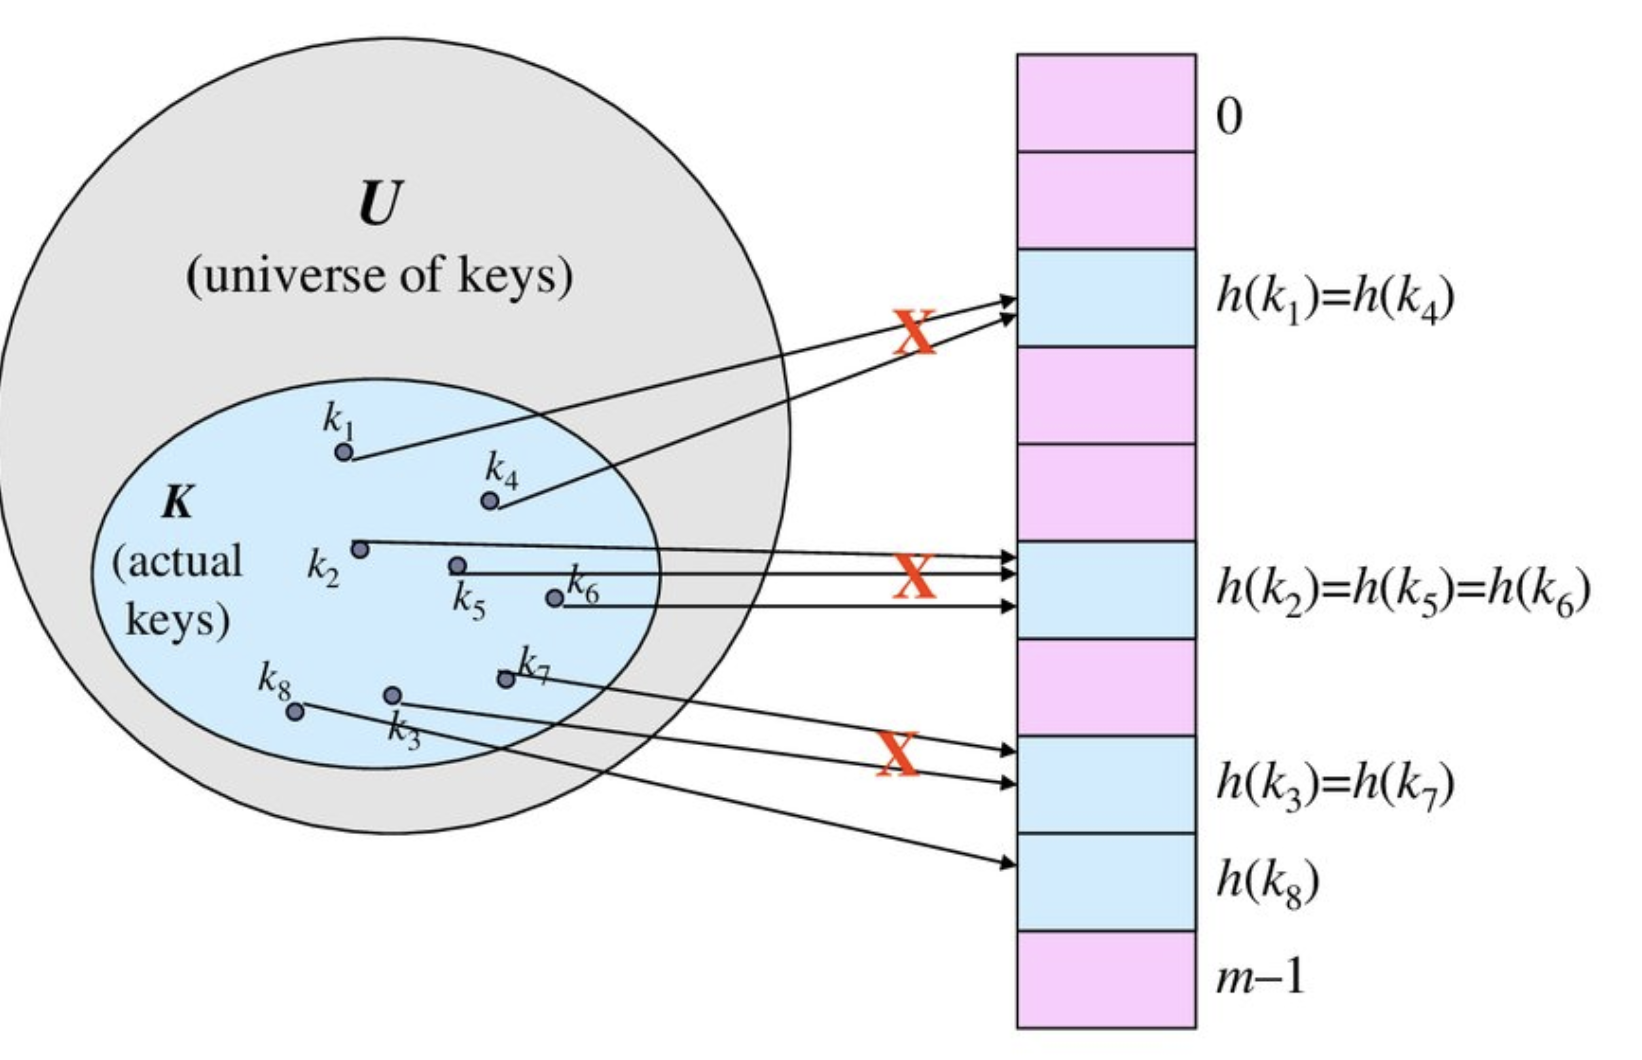
\includegraphics[width=0.8\textwidth]{aulas/aula2-hash-fig2.png}
    \caption{Tratamento de Colisões}
  \end{figure}
\end{frame}

% Slide 2: Métodos de Tratamento de Colisões

\begin{frame}[fragile]
  \frametitle{Métodos de Tratamento de Colisões}
  \begin{itemize}
    \item Encadeamento externo:
      \begin{itemize}
        \item No método de encadeamento externo, cada entrada da tabela de dispersão mantém uma lista encadeada de todos os elementos que colidem naquele índice específico.
        \item Quando ocorre uma colisão, o novo elemento é simplesmente adicionado à lista encadeada correspondente.
        \item Este método é simples de implementar e eficaz para lidar com colisões, especialmente em cenários onde as colisões são frequentes.
        \item No entanto, pode exigir mais espaço de memória devido à necessidade de armazenar as listas encadeadas.
      \end{itemize}
  \end{itemize}
\end{frame}

\begin{frame}[fragile]
  \frametitle{Tratamento de Colisões - Encadeamento}
  \begin{figure}
    \centering
    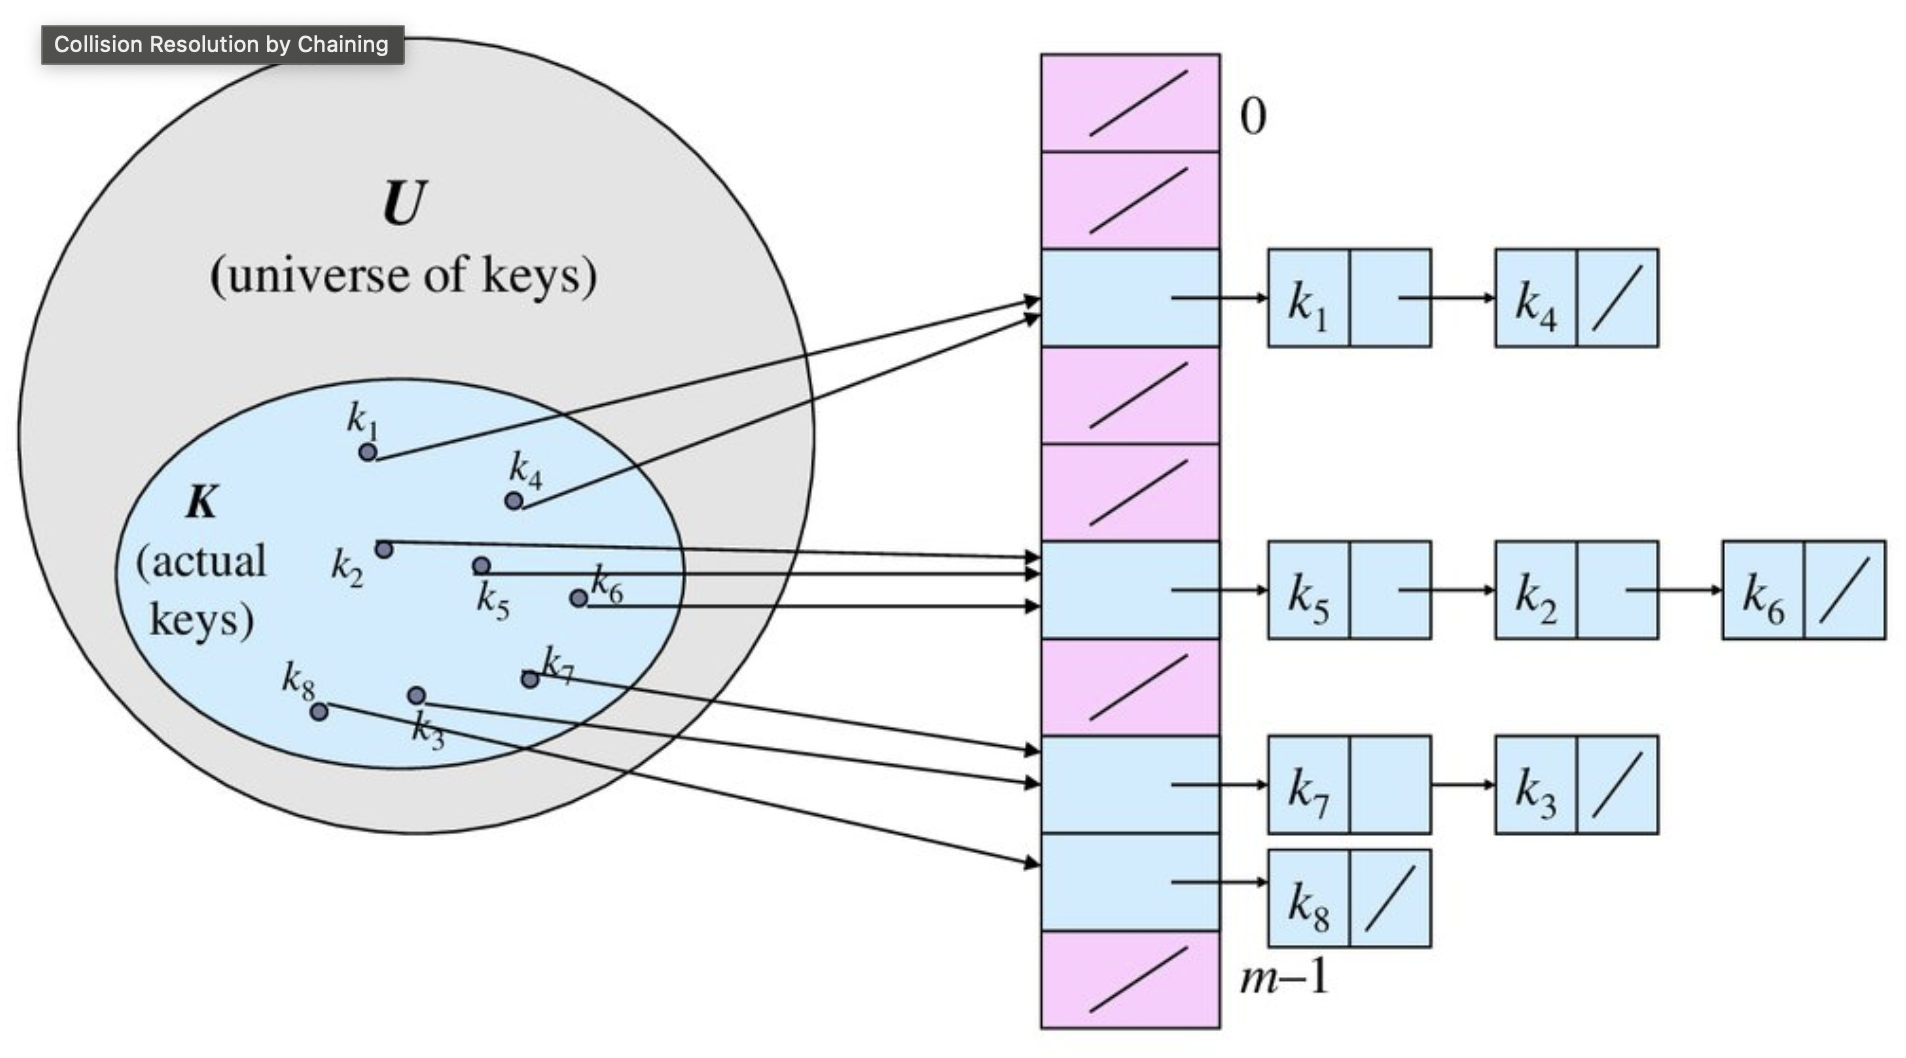
\includegraphics[width=0.8\textwidth]{aulas/aula2-hash-fig3.png}
    \caption{Tratamento de Colisões}
  \end{figure}
\end{frame}


\begin{frame}[fragile]
  \frametitle{Métodos de Tratamento de Colisões}
  \begin{itemize}
    \item Endereçamento aberto:
      \begin{itemize}
        \item O endereçamento aberto é uma abordagem em que, quando ocorre uma colisão, a tabela de dispersão é pesquisada por outra posição livre para inserir o novo elemento.
        \item Existem várias técnicas de endereçamento aberto, incluindo sondagem linear, sondagem quadrática e hashing duplo.
        \item Estas técnicas diferem na forma como procuram por posições alternativas na tabela quando ocorre uma colisão.
        \item O endereçamento aberto pode ser mais eficiente em termos de uso de memória, mas requer cuidados especiais para evitar clusters de colisões.
      \end{itemize}
  \end{itemize}
\end{frame}


% Slide 3: Exemplos e Análise de Métodos de Tratamento de Colisões

\begin{frame}[fragile]
  \frametitle{Exemplos e Análise de Métodos de Tratamento de Colisões}
Comparação dos métodos de tratamento de colisões:
      \begin{itemize}
        \item Encadeamento externo:
          \begin{itemize}
            \item No método de encadeamento externo, as colisões são tratadas armazenando múltiplos elementos que colidem no mesmo índice em uma estrutura de dados separada, como uma lista encadeada.
            \item Vantagens:
              \begin{itemize}
                \item Fácil implementação.
                \item Eficiente para lidar com colisões frequentes.
              \end{itemize}
            \item Desvantagens:
              \begin{itemize}
                \item Pode consumir mais espaço de memória devido à necessidade de armazenar listas encadeadas.
                \item Pode levar a acessos indiretos adicionais durante a busca de elementos.
              \end{itemize}
          \end{itemize}
      \end{itemize}
\end{frame}

\begin{frame}[fragile]
  \frametitle{Exemplos e Análise de Métodos de Tratamento de Colisões (Continuação)}
Comparação dos métodos de tratamento de colisões (cont.):
      \begin{itemize}
        \item Endereçamento aberto:
          \begin{itemize}
            \item No endereçamento aberto, quando ocorre uma colisão, novas posições na tabela de dispersão são pesquisadas para encontrar um local alternativo para o novo elemento.
            \item Vantagens:
              \begin{itemize}
                \item Mais eficiente em termos de uso de memória, pois não requer estruturas de dados adicionais.
                \item Pode ser mais rápido em alguns cenários, especialmente quando as colisões são raras.
              \end{itemize}
            \item Desvantagens:
              \begin{itemize}
                \item Requer técnicas adicionais para lidar com clusters de colisões.
                \item Pode ser mais complicado de implementar.
              \end{itemize}
          \end{itemize}
      \end{itemize}
\end{frame}

\begin{frame}[fragile]
  \frametitle{Exemplos e Análise de Métodos de Tratamento de Colisões (Continuação)}
  Discussão sobre as vantagens e desvantagens de cada método:
  \begin{itemize}
    \item A escolha entre encadeamento externo e endereçamento aberto 
    depende das características específicas do problema, como a 
    distribuição das chaves e a frequência de colisões.
  \end{itemize}
\end{frame}

% Slide 4: Prática - Implementando e Testando o Tratamento de Colisões
\begin{frame}[fragile]
  \frametitle{Prática - Implementando e Testando o Tratamento de Colisões (Parte 1)}
  \begin{verbatim}
    // Exemplo de encadeamento externo em pseudocódigo
    inserir(chave, valor):
      indice = funcao_hash(chave)
      se tabela[indice] não está vazia:
        inserir na lista encadeada
      senão:
        criar nova entrada
  \end{verbatim}
  \begin{itemize}
    \item Atividade prática: Implementação e testes com diferentes cenários de colisões.
  \end{itemize}
\end{frame}

\begin{frame}[fragile]
  \frametitle{Prática - Implementando e Testando o Tratamento de Colisões (Parte 2)}
  \textbf{Exemplo de Encadeamento Externo:}
  \begin{itemize}
    \item Suponha que temos uma tabela de dispersão de tamanho 5 e a seguinte sequência de chaves é inserida: 7, 12, 3, 8, 18.
    \item A função hash poderia ser algo como "chave \% 5".
    \item Quando ocorre uma colisão, inserimos na lista encadeada correspondente.
  \end{itemize}
\end{frame}
\begin{frame}[fragile]
  \frametitle{Prática - Implementando e Testando o Tratamento de Colisões (Parte 3)}
  \textbf{Exemplo de Endereçamento Aberto:}
  \begin{itemize}
    \item Suponha a mesma tabela de dispersão de tamanho 5 e a mesma sequência de chaves é inserida.
    \item A função hash poderia ser "chave \% 5".
    \item Quando ocorre uma colisão, procuramos por uma posição alternativa na tabela para inserir a chave.
  \end{itemize}
\end{frame}

\begin{frame}[fragile]{Descrição do Problema: Soma Dois}
O problema "Soma Dois" (Two Sum) é um desafio de codificação clássico 
usado em entrevistas de emprego e prática de algoritmos. O objetivo é 
encontrar dois números em um array de inteiros que somem um valor alvo 
específico.

Requisitos:
\begin{itemize}
  \item Dado um array de inteiros `numeros` e um inteiro `alvo`.
  \item Retornar os índices dos dois números de tal forma que eles somem ao `alvo`.
  \item Você pode assumir que cada entrada teria exatamente uma solução, e você não pode usar o mesmo elemento duas vezes.
  \item A resposta pode ser retornada em qualquer ordem.
\end{itemize}

\end{frame}
\begin{frame}{Descrição das Entradas e Saídas}
  \textbf{Entradas:}
  \begin{itemize}
      \item Um \textit{array} de inteiros \texttt{numeros}.
      \item Um inteiro \texttt{alvo}, representando o valor alvo a ser alcançado pela soma de dois números no array.
  \end{itemize}
  
  \textbf{Saídas:}
  \begin{itemize}
      \item Uma lista contendo os índices dos \textit{dois números} dentro do array \texttt{numeros} que somam para o valor \texttt{alvo}.
  \end{itemize}
  
  \textbf{Exemplo:}
  \begin{itemize}
      \item \textbf{Entrada:} \texttt{numeros = [2, 7, 11, 15]}, \texttt{alvo = 9}
      \item \textbf{Saída:} \texttt{[0, 1]}
      \item \textbf{Explicação:} \texttt{numeros[0] + numeros[1] == 9}, portanto, retornamos \texttt{[0, 1]}.
  \end{itemize}
\end{frame}
\begin{frame}{Casos de Teste}
  \begin{block}{Caso de Teste 1}
      \textbf{Entrada:} \texttt{numeros = [2, 7, 11, 15]}, \texttt{alvo = 9}\\
      \textbf{Saída esperada:} \texttt{[0, 1]}
  \end{block}

  \begin{block}{Caso de Teste 2}
      \textbf{Entrada:} \texttt{numeros = [3, 2, 4]}, \texttt{alvo = 6}\\
      \textbf{Saída esperada:} \texttt{[1, 2]}
  \end{block}

  \begin{block}{Caso de Teste 3}
      \textbf{Entrada:} \texttt{numeros = [3, 3]}, \texttt{alvo = 6}\\
      \textbf{Saída esperada:} \texttt{[0, 1]}
  \end{block}

  \begin{block}{Caso de Teste 4}
      \textbf{Entrada:} \texttt{numeros = [-1, -2, -3, -4, -5]}, \texttt{alvo = -8}\\
      \textbf{Saída esperada:} \texttt{[2, 4]}
  \end{block}
\end{frame}
\begin{frame}[fragile]{Solução do problema "Dois Soma" em JavaScript}
  \small
  \begin{lstlisting}
  function somaDois(numeros, alvo) {
      // Inicializa um objeto para mapear os numeros aos seus indices
      let mapa = {}; 
      for (let i = 0; i < numeros.length; i++) {
        // Calcula o complemento do numero atual
          const complemento = alvo - numeros[i]; 
          // Verifica se o complemento já existe no mapa
          if (mapa[complemento] !== undefined) {
            // Retorna os indices do complemento e do numero atual    
          return [mapa[complemento], i]; 
          }
          // Adiciona o numero atual ao mapa com seu indice
          mapa[numeros[i]] = i; 
      }
      // Retorna uma lista vazia se nenhum par for encontrado
      return []; 
  }
  \end{lstlisting}
\end{frame}

\begin{frame}[fragile]{Contexto do Problema}
  Imagine o restaurante "Sabor e Arte", famoso pela sua cozinha inovadora e diversificada. A cada mês, o restaurante introduz novos pratos ao menu, buscando surpreender e satisfazer seus clientes. Para entender melhor quais pratos são os mais apreciados, o restaurante coleta avaliações dos clientes, que vão de 0 a 5 estrelas.
  
  Com o aumento do número de avaliações, tornou-se desafiador para a equipe do restaurante identificar rapidamente quais pratos estão fazendo mais sucesso. Eles precisam de uma solução que calcule automaticamente a média das avaliações de cada prato e destaque o prato com a melhor média. Em caso de empate nas médias, o prato introduzido mais recentemente (assumindo que tem o ID mais alto) deve ser considerado o menos favorito, como forma de incentivar a inovação constante.
  
  O desafio é desenvolver um algoritmo que ajude o "Sabor e Arte" a reconhecer o prato estrela de cada mês, otimizando sua oferta e garantindo a satisfação dos clientes.
\end{frame}
    

  \begin{frame}[fragile]{Descrição do Problema e Restrições}
    \begin{itemize}
        \item Dado um array de pares, onde cada par consiste em um identificador de produto (\texttt{id}) e uma avaliação dada por um cliente (\texttt{rating}).
        \item Os \texttt{id} dos produtos variam de 1 a 5000.
        \item As avaliações (\texttt{rating}) variam de 0 a 5.
        \item O objetivo é calcular a média das avaliações de cada produto.
        \item Deve-se retornar o produto com a maior avaliação média.
        \item Se dois produtos possuírem a mesma média, retorna o produto com o ID menor.
    \end{itemize}
\end{frame}

\begin{frame}[fragile]{Casos de Teste Adicionais}
  \textbf{Caso de Teste 4:} 8 elementos\
  Entrada: \texttt{[[4001, 3], [4002, 2], [4001, 4], [4003, 5], [4001, 5], [4004, 1], [4005, 4], [4001, 3]]}\
  Saída esperada: \texttt{4001}
  
  \textbf{Caso de Teste 5:} 6 elementos\
  Entrada: \texttt{[[5001, 5], [5002, 5], [5003, 3], [5004, 3], [5002, 4], [5001, 4]]}\
  Saída esperada: \texttt{5001} \textit{(5001 tem id menor que 5002)}
  
  \textbf{Caso de Teste 6:} 4 elementos\
  Entrada: \texttt{[[6001, 1], [6002, 2], [6003, 3], [6004, 4]]}\
  Saída esperada: \texttt{6004}
  \end{frame}

\begin{frame}[fragile]{Solução em JavaScript}
  \begin{lstlisting}[language=JavaScript]
  function encontrarMelhorAvaliacao(avaliacoes) {
      const somaAvaliacoes = {};
      const contagemAvaliacoes = {};
      avaliacoes.forEach(([id, rating]) => {
          if (somaAvaliacoes[id]) {
              somaAvaliacoes[id] += rating;
              contagemAvaliacoes[id] += 1;
          } else {
              somaAvaliacoes[id] = rating;
              contagemAvaliacoes[id] = 1;
          }
      });
      ...
  }
  \end{lstlisting}
\end{frame}
\begin{frame}[fragile]{Solução em JavaScript}
  \begin{lstlisting}[language=JavaScript]
  function encontrarMelhorAvaliacao(avaliacoes) {
      ...
      let melhorId = null;
      let maiorMedia = 0;
      for (const id in somaAvaliacoes) {
          const media = somaAvaliacoes[id] / contagemAvaliacoes[id];
          if (media > maiorMedia || (media === maiorMedia && (melhorId === null || parseInt(id) < melhorId))) {
              maiorMedia = media;
              melhorId = id;
          }
      }
      return melhorId;
  }
  \end{lstlisting}
  \end{frame}
  
\begin{frame}[fragile]{Agrupamento de Anagramas}
  Escreva uma função que receba um array de strings e agrupe os anagramas.
  
  Anagramas são strings compostas pelas mesmas letras, onde a ordem não importa. Por exemplo, \texttt{"cinema"} e \texttt{"iceman"} são anagramas; da mesma forma, \texttt{"foo"} e \texttt{"ofo"} são anagramas.
  
  A função deve retornar uma lista de grupos de anagramas em qualquer ordem.

  \textbf{Entrada de Exemplo:}\\
  \texttt{words = ["yo", "act", "flop", "tac", "foo", "cat", "oy", "olfp"]}

  \textbf{Saída de Exemplo:}\\
  \texttt{{[["yo", "oy"], ["flop", "olfp"], ["act", "tac", "cat"], ["foo"]}}
\end{frame}
  
\title{Introdução às Listas Ligadas}
\date{\today}
\frame{\titlepage}

% Slide 1: Flexibilidade de Memória
\begin{frame}[fragile]
  \frametitle{Flexibilidade de Memória}
  \begin{itemize}
  \item \textbf{Alocação Dinâmica:} Diferentemente dos vetores, que precisam de um tamanho definido na sua criação, listas ligadas permitem alocação dinâmica de memória.
  \item \textbf{Crescimento Incremental:} É possível adicionar novos nós à lista ligada sem a necessidade de realocação ou cópia de dados, ao contrário dos vetores, que podem exigir realocação e cópia de todo o array quando o espaço alocado inicialmente é excedido.
  \item \textbf{Eficiência de Espaço:} Com listas ligadas, a memória é alocada conforme a necessidade. Isso contrasta com vetores, onde é comum alocar mais memória do que o necessário para acomodar o crescimento futuro, o que pode levar a uma utilização ineficiente da memória.
  \end{itemize}
  \end{frame}
  
  % Slide 2: Inserção e Remoção Eficientes
  \begin{frame}[fragile]
  \frametitle{Inserção e Remoção Eficientes}
  \begin{itemize}
  \item \textbf{Complexidade de Tempo:} A inserção e a remoção de elementos em uma lista ligada podem ser feitas com tempo constante ( O(1)), assumindo que temos um ponteiro direto para o local de inserção/remoção. Em comparação, essas operações em vetores podem requerer tempo linear (O(n)) devido à necessidade de deslocar elementos.
  \item \textbf{Flexibilidade:} Listas ligadas permitem inserções e remoções em qualquer ponto da lista com eficiência, tornando-as ideais para aplicações que requerem manipulação frequente de dados.
  \item \textbf{Sem Deslocamento Necessário:} Ao contrário dos vetores, onde a inserção ou remoção de elementos pode requerer o deslocamento de muitos elementos, listas ligadas simplesmente requerem a atualização dos ponteiros.
  \end{itemize}
  \end{frame}
  
  % Slide 3: Comparação de Acesso aos Elementos
  \begin{frame}[fragile]
  \frametitle{Comparação de Acesso aos Elementos}
  \begin{itemize}
  \item \textbf{Acesso Direto vs. Sequencial:} Vetores oferecem acesso direto a qualquer elemento através de índices, o que é uma grande vantagem para buscas rápidas ( O(1)). Em contraste, listas ligadas requerem acesso sequencial aos elementos ( O(n)), o que pode ser menos eficiente para buscas.
  \item \textbf{Aplicações Adequadas:} Devido à diferença no acesso aos elementos, listas ligadas são preferíveis em cenários onde as operações de inserção e remoção são mais comuns do que a busca direta por elementos.
  \item \textbf{Decisão Baseada no Uso:} A escolha entre listas ligadas e vetores deve ser guiada pelo tipo de operações que serão mais frequentes na aplicação, levando em consideração as trade-offs entre acesso rápido e eficiência de inserção/remoção.
  \end{itemize}
  \end{frame}

  % Slide: O Que é um Nó?
\begin{frame}[fragile]
  \frametitle{O Que é um Nó?}
  \begin{itemize}
    \item \textbf{Componente Fundamental:} Um nó é o bloco de construção básico de uma lista ligada.
    \item \textbf{Estrutura:} Consiste em pelo menos dois elementos:
      \begin{itemize}
        \item \textit{Dados:} O valor ou informação que o nó armazena.
        \item \textit{Ponteiro(s):} Um ou mais ponteiros que ligam este nó ao próximo nó na lista (e possivelmente ao anterior, em listas duplamente ligadas).
      \end{itemize}
    \item \textbf{Finalidade:} Permite a criação de estruturas de dados lineares, dinâmicas e não contíguas.
    \item \textbf{Flexibilidade:} Os nós podem ser facilmente inseridos ou removidos, alterando apenas os ponteiros, sem necessidade de realocação de outros elementos.
  \end{itemize}
\end{frame}

\begin{frame}[fragile]
  \frametitle{Nó}
  \begin{figure}
    \centering
    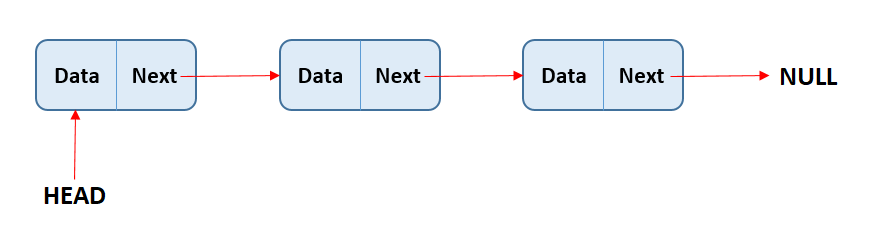
\includegraphics[width=0.8\textwidth]{aulas/aula3-lista-ligada1.png}
    \caption{Um nó}
  \end{figure}
\end{frame}

% Slide: Definição de Nó em C (Struct)
\begin{frame}[fragile]
  \frametitle{Definição de Nó em C (Struct)}
  \begin{lstlisting}[language=C]
typedef struct Node {
    int data; // Dados armazenados no nó
    struct Node* next; // Ponteiro para o próximo nó
} Node;
  \end{lstlisting}
  \begin{itemize}
    \item Esta \texttt{struct} define um nó de uma lista ligada simples em C.
    \item \texttt{data} armazena o valor do nó.
    \item \texttt{next} é um ponteiro para o próximo nó na lista, permitindo a ligação entre os nós.
  \end{itemize}
\end{frame}

% Slide: Definição de Nó em JavaScript/TypeScript
\begin{frame}[fragile]
  \frametitle{Definição de Nó em JavaScript/TypeScript}
  \begin{lstlisting}[language=JavaScript]
class Node {
    constructor(public data: number, public next: Node | null = null) {}
}
  \end{lstlisting}
  \begin{itemize}
    \item Esta classe define um nó de uma lista ligada em JavaScript/TypeScript.
    \item \texttt{data} é a propriedade que armazena o valor do nó.
    \item \texttt{next} é uma propriedade que aponta para o próximo nó na lista, inicialmente nulo se não especificado.
    \item A sintaxe \texttt{public} no construtor automaticamente declara e inicializa as propriedades da classe.
  \end{itemize}
\end{frame}

% Tipos de Listas Ligadas
% Slide: Lista Ligada Simples
\begin{frame}[fragile]
  \frametitle{Lista Ligada Simples}
  \begin{itemize}
    \item \textbf{Definição:} Uma lista ligada simples consiste em nós onde cada nó tem um ponteiro que aponta para o próximo nó na sequência.
    \item \textbf{Terminação:} O último nó aponta para NULL, indicando o fim da lista.
    \item \textbf{Operações:} Suporta operações básicas como inserção, remoção e travessia de forma eficiente, principalmente quando se trabalha no início da lista.
    \item \textbf{Uso:} Ideal para implementações simples onde a travessia é majoritariamente feita em uma única direção.
  \end{itemize}
\end{frame}

\begin{frame}[fragile]
  \frametitle{Lista ligada}
  \begin{figure}
    \centering
    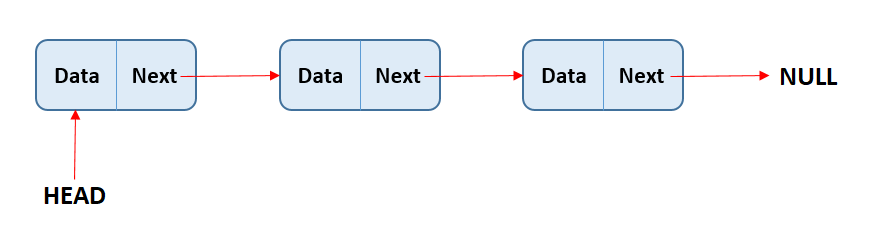
\includegraphics[width=0.8\textwidth]{aulas/aula3-lista-ligada1.png}
    \caption{Lista ligada}
  \end{figure}
\end{frame}
% Slide: Lista Duplamente Ligada
\begin{frame}[fragile]
  \frametitle{Lista Duplamente Ligada}
  \begin{itemize}
    \item \textbf{Definição:} Em uma lista duplamente ligada, cada nó contém dois ponteiros, um apontando para o próximo nó e outro para o anterior.
    \item \textbf{Flexibilidade:} Permite travessia nos dois sentidos (para frente e para trás), facilitando operações como reversão da lista e remoção de nós.
    \item \textbf{Uso de Memória:} Requer mais memória por nó em comparação com a lista ligada simples devido aos ponteiros extras.
    \item \textbf{Aplicações:} Útil em aplicações que necessitam de travessias bidirecionais ou inserções/remoções eficientes em qualquer ponto da lista.
  \end{itemize}
\end{frame}

\begin{frame}[fragile]
  \frametitle{Lista duplamente ligada}
  \begin{figure}
    \centering
    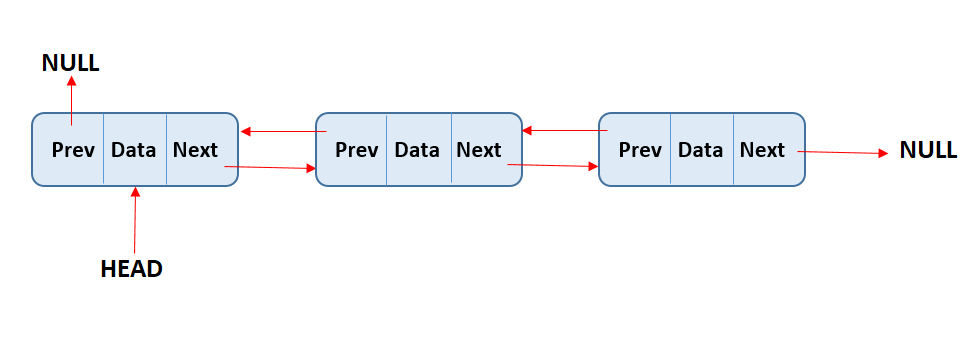
\includegraphics[width=0.8\textwidth]{aulas/aula3-dll.png}
    \caption{DLL}
  \end{figure}
\end{frame}
% Slide: Lista Circular
\begin{frame}[fragile]
  \frametitle{Lista Circular}
  \begin{itemize}
    \item \textbf{Definição:} Uma variação da lista ligada onde o último nó aponta de volta para o primeiro nó, formando um círculo.
    \item \textbf{Característica:} Não tem um fim claro como as listas ligadas simples ou duplamente ligadas, permitindo travessia contínua pela lista.
    \item \textbf{Considerações:} A implementação e a manutenção podem ser mais complexas, especialmente em listas circulares duplamente ligadas.
    \item \textbf{Uso:} Ideal para aplicações que necessitam de um ciclo contínuo de elementos, como algoritmos de round robin.
  \end{itemize}
\end{frame}

\begin{frame}[fragile]
  \frametitle{Lista circular}
  \begin{figure}
    \centering
    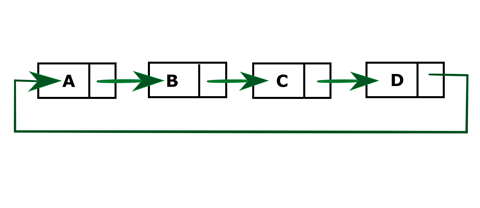
\includegraphics[width=0.8\textwidth]{aulas/aula3-cll.png}
    \caption{Lista circular}
  \end{figure}
\end{frame}

% Operações Básicas
\begin{frame}[fragile]
\frametitle{Operações Básicas}
\begin{itemize}
\item \textbf{Inserção:} Adiciona um novo nó à lista.
\begin{itemize}
\item No início, no meio, ou no fim da lista.
\end{itemize}
\item \textbf{Remoção:} Remove um nó da lista.
\begin{itemize}
\item Requer a atualização dos ponteiros do nó anterior e/ou posterior.
\end{itemize}
\item \textbf{Busca:} Encontra um nó na lista.
\begin{itemize}
\item Pode ser realizada iterando-se através dos nós até encontrar o desejado.
\end{itemize}
\item \textbf{Travessia:} Acessa cada nó da lista sequencialmente.
\end{itemize}
\end{frame}
% Slide: Inserção em Lista Ligada
\begin{frame}[fragile]
  \frametitle{Inserção em Lista Ligada}
  \begin{block}{Descrição}
    Adiciona um novo nó à lista. Pode ser realizado no início, no meio ou no fim da lista.
  \end{block}
  \small
  \begin{block}{Código em Portugol}
    procedimento inserirNoInicio(lista, valor) \\
    inicio \\
    \ \ novoNo := novo Nó \\
    \ \ novoNo.dado := valor \\
    \ \ novoNo.proximo := lista.cabeca \\
    \ \ lista.cabeca := novoNo \\
    fim
  \end{block}
\end{frame}

% Slide: Remoção em Lista Ligada
\begin{frame}[fragile]
  \frametitle{Remoção em Lista Ligada}
  \begin{block}{Descrição}
    Remove um nó da lista. Requer a atualização dos ponteiros do nó anterior (se houver) para apontar para o próximo nó do que está sendo removido.
  \end{block}
  
\end{frame}
\begin{frame}[fragile]
  \frametitle{Remoção em Lista Ligada - Código em Portugol}
  \small
  \begin{block}{Código em Portugol}
    procedimento removerNo(lista, valor) \\
    inicio \\
    \ \ se lista.cabeca = nulo então retorne fimSe \\
    \ \ se lista.cabeca.dado = valor então \\
    \ \ \ \ lista.cabeca := lista.cabeca.proximo \\
    \ \ senao \\
    \ \ \ \ atual := lista.cabeca \\
    \ \ \ \ enquanto atual.proximo ≠ nulo e atual.proximo.dado ≠ valor faça \\
    \ \ \ \ \ \ atual := atual.proximo \\
    \ \ \ \ fimEnquanto \\
    \ \ \ \ se atual.proximo ≠ nulo então \\
    \ \ \ \ \ \ atual.proximo := atual.proximo.proximo \\
    \ \ \ \ fimSe \\
    \ \ fimSe \\
    fim
  \end{block}
\end{frame}

% Slide: Busca em Lista Ligada
\begin{frame}[fragile]
  \frametitle{Busca em Lista Ligada}
  \begin{block}{Descrição}
    Encontra um nó na lista. A busca é realizada iterando-se através dos nós até encontrar o desejado.
  \end{block}
  \small
  \begin{block}{Código em Portugol}
    funcao buscarNo(lista, valor) : Nó \\
    inicio \\
    \ \ atual := lista.cabeca \\
    \ \ enquanto atual ≠ nulo faça \\
    \ \ \ \ se atual.dado = valor então \\
    \ \ \ \ \ \ retorne atual \\
    \ \ \ \ fimSe \\
    \ \ \ \ atual := atual.proximo \\
    \ \ fimEnquanto \\
    \ \ retorne nulo \\
    fim
  \end{block}
\end{frame}

% Slide: Travessia em Lista Ligada
\begin{frame}[fragile]
  \frametitle{Travessia em Lista Ligada}
  \begin{block}{Descrição}
    Acessa cada nó da lista sequencialmente. Utilizado para imprimir todos os elementos, ou para aplicar uma função a cada elemento da lista.
  \end{block}
  \small
  \begin{block}{Código em Portugol}
    procedimento percorrerLista(lista) \\
    inicio \\
    \ \ atual := lista.cabeca \\
    \ \ enquanto atual ≠ nulo faça \\
    \ \ \ \ escreva(atual.dado) \\
    \ \ \ \ atual := atual.proximo \\
    \ \ fimEnquanto \\
    fim
  \end{block}
\end{frame}

% Vantagens e Desvantagens
\begin{frame}[fragile]
\frametitle{Vantagens e Desvantagens}
\begin{itemize}
\item \textbf{Vantagens:}
\begin{itemize}
\item Flexibilidade no tamanho.
\item Inserção e remoção eficientes.
\end{itemize}
\item \textbf{Desvantagens:}
\begin{itemize}
\item Acesso sequencial (não aleatório) aos elementos.
\item Maior uso de memória devido aos ponteiros.
\end{itemize}
\end{itemize}
\end{frame}



\end{document}
